

\documentclass{beamer}
\usetheme{CambridgeUS}
\mode<presentation>
{
\setbeamercovered{transparent}
}
\usepackage{amsmath,amsfonts,amssymb}
\usepackage{german}
\usepackage[center]{caption}
\usepackage[utf8]{inputenc}
\usepackage[ngerman]{babel}
\usepackage{graphicx}
\usepackage{svg}
\usepackage{pdfpages}
\usepackage{placeins}
\usepackage[decimalsymbol=comma]{siunitx}


% font definitions, try \usepackage{ae} instead of the following
% three lines if you don't like this look
\usepackage{mathptmx}
\usepackage[scaled=.90]{helvet}
\usepackage{courier}
\beamertemplatenavigationsymbolsempty 
\setbeamertemplate{footline}{}

%\usepackage[T1]{fontenc}
\title[Bachelorarbeit]{Untersuchung des Wachstums von Au auf Re(0001) mittels LEED und STM sowie
Aufbau und Test einer Spraydepositionsapparatur}
\author[V. Grimm]{Verena Grimm}


\institute[]{
Vortrag zur Bachelorarbeit in Physik\\
Fachbereich Physik, Mathematik und Informatik (FB 08)\\
Johannes Gutenberg-Universität Mainz
}

\date{00.00.2014}


% Logo Universität
\titlegraphic{
\includegraphics[width=4cm]{bilder/JGU-Logo_sw_high.jpg}\hspace*{-8.5cm}}
% Logo auf jeder Seite rechts unten:
% \pgfdeclareimage[height=1.5cm]{university-logo}{bilder/JGU-Logo_sw_high.jpg}
%  \logo{\pgfuseimage{university-logo}}



\begin{document}

\begin{frame}
\titlepage
\end{frame}

\begin{frame}
\frametitle{Inhalt}
\tableofcontents
% You might wish to add the option [pausesections]
\end{frame}



%___________________________________________________________________________________________________________________________________________
%___________________________________________________________________________________________________________________________________________
%___________________________________________________________________________________________________________________________________________



\section{Wachstum von Au auf Re(0001)}

%___________________________________________________________________________________________________________________________________________
%___________________________________________________________________________________________________________________________________________


\begin{frame}
\frametitle{}
%\framesubtitle{Subtitles are optional}
\begin{center}
\textcolor{darkred}{\huge{1. Teil:\\ \vspace{0.5cm}
Untersuchung des Wachstums von Au \\ \vspace{0.5cm} auf Re(0001)}}
\end{center}
\end{frame}

%___________________________________________________________________________________________________________________________________________
%___________________________________________________________________________________________________________________________________________


\subsection[Motivation]{Motivation}

\begin{frame}
\frametitle{Warum Gold? Warum Rhenium?}
%\framesubtitle{Subtitles are optional}
\begin{itemize}\setlength{\itemsep}{+15pt}
 	\item Gold inert, d.h. wenig Reaktion mit Restgasmolekülen im Ultrahochvakuum
 	\item gute Adsorption organischer Moleküle auf Goldoberflächen
 \end{itemize}
 \vspace{1cm}
 \begin{itemize}\setlength{\itemsep}{+15pt}
  	\item Rhenium: hoher Schmelzpunkt ($3186^\circ$C)
  	\item bleibt nach Verarbeitung (Schweißen, Schmieden, \ldots) duktil
 \end{itemize}
\end{frame}

%___________________________________________________________________________________________________________________________________________
%___________________________________________________________________________________________________________________________________________


\subsection[Grundlagen]{Grundlagen: STM und LEED}

\begin{frame}
\frametitle{LEED (Low Energy Electron Diffraction)}
\framesubtitle{Beugung niederenergetischer Elektronen an Oberflächen}
\begin{figure}[htbp]
	\begin{minipage}[b]{0.45\textwidth}
		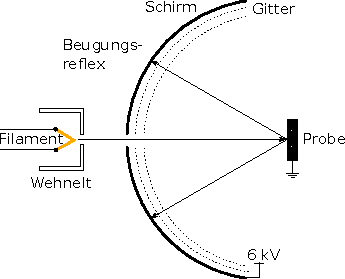
\includegraphics[]{bilder/leedkleiner}
	\end{minipage}
	\hspace{0.4cm}
	\begin{minipage}[b]{0.45\textwidth}
		\begin{itemize}
 		\item Elektronenstrahl durch Glühemission mit \SI{20}{eV} bis \SI{400}{eV}
 	 	\item niedrige Eindringtiefe der Elektronen
 	 	\item Fokussierung und "`Sortierung"' durch Gitter vor Schirm
 	 	\item betrachte elastisch rückgestreute Elektronen auf fluoreszierendem Schirm
		\end{itemize}
	\end{minipage}
\end{figure}
\end{frame}

\begin{frame}
\frametitle{LEED (Low Energy Electron Diffraction)}
\begin{figure}[H]
\begin{minipage}[b]{0.45\textwidth}
		\begin{itemize}
 		\item Betrachte elastische Streuung an oberster Schicht mit $k=k'$
 	 	\item konstruktive Interferenz allgemein, wenn $\vec{k}-\vec{k'}=\Delta \vec{k}=\vec{G}$~~~und
 	 	$\vec{a}_i\cdot \Delta \vec{k}=2\pi h_i,~~~~~~~i=1, 2, 3$
 	 	\item bei Oberflächenstreuung: $\Delta\vec{k}_{||}=\vec{k}_{||}-\vec{k'}_{||}\overset{!}{=} \vec{G}$
 	 	\item in Ewald-Konstruktion werden Punkten $(h_1, h_2)$ Linien $h_3$ zugeordnet
 	 	\item Schnittstellen Linien-Kugel: Interferenz!
		\end{itemize}
	\end{minipage}
	\hspace{0.4cm}
	\begin{minipage}[b]{0.45\textwidth}
		\includesvg[svgpath=bilder/]{ewald}
	\end{minipage}
\end{figure}
\end{frame}




\begin{frame}
\frametitle{STM (Scanning Tunneling Microscope)}
\framesubtitle{Rastertunnelmikroskopie}
\begin{itemize}\setlength{\itemsep}{+15pt}
  \item 3D Aufnahme von Oberflächen elektrisch leitender Festkörper
  \item Annäherung leitender Spitze an Oberfläche bis auf wenige {\AA} $\Rightarrow$ mit angelegter
  Spannung fließt messbarer Strom
  \item Mechanismus beruht auf Tunneleffekt
  \item Rastern der Oberfläche mit Spitze bei Messung des Stroms: topographisches Bild der
  Oberfläche mit atomarer Auflösung
\end{itemize}
\end{frame}

\begin{frame}
\frametitle{STM (Scanning Tunneling Microscope)}
	 \begin{columns}
\column{.45\textwidth}
\begin{figure}[H]
\begin{center}
\begin{itemize}\setlength{\itemsep}{+15pt}
		  \item Berechnungen schwer durch i.A. unbekannte Wellenfunktion der Spitze
		  \item Ausdruck für Strom nur durch Näherungen erreichbar
		  \item $I\propto U \rho_{s}(E_F) \rho_P(\vec{r}_0, E)e^{-2\kappa d}$
		\end{itemize}
\end{center}
\end{figure}

   \column{.45\textwidth}
\begin{figure}[H]
\begin{center}
\includesvg[svgpath=bilder/]{spitze}
\end{center}
\end{figure}
\end{columns}
\end{frame}

%___________________________________________________________________________________________________________________________________________
%___________________________________________________________________________________________________________________________________________


\subsection[Versuchsaufbau]{Versuchsaufbau}

\begin{frame}
\frametitle{Versuchsaufbau}
\begin{itemize}\setlength{\itemsep}{+15pt}
  \item UHV-Apparatur mit \SI{e-10}{mbar}
  \item Flashen, Tempern, Bedampfen der Probe mit Gold
  \item Bestimmung der aufgedampften Menge über Schwingquarz
  \item LEED, STM
\end{itemize}
\end{frame}

\begin{frame}
\frametitle{Aufbau der UHV-Apparatur}
\begin{figure}[H]
\centering
\sffamily
\includesvg[svgpath=bilder/]{uhv-apparatur}
\end{figure}
\end{frame}

\begin{frame}
\frametitle{Das STM}
\begin{figure}[H]
\centering
\sffamily
\includesvg[svgpath=bilder/]{stm-tisch}
\end{figure}
\end{frame}

%___________________________________________________________________________________________________________________________________________
%___________________________________________________________________________________________________________________________________________


\subsection[Ergebnisse]{LEED}

\begin{frame}
\frametitle{LEED des Re-Kristalls}
\begin{figure}[htbp]
	\begin{minipage}[b]{0.45\textwidth}
	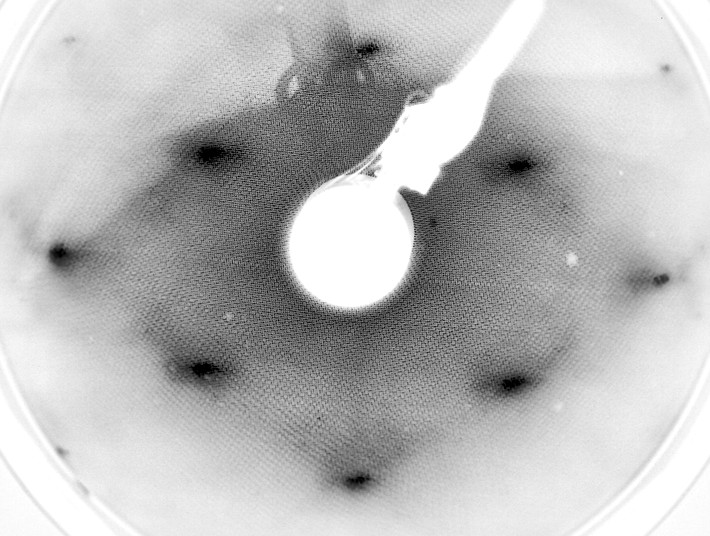
\includegraphics[width=\textwidth]{bilder/unbedampft_E207}
	\caption*{Rand des Kristalls}
	\end{minipage}
	\hspace{0.2cm}
	\begin{minipage}[b]{0.45\textwidth}
	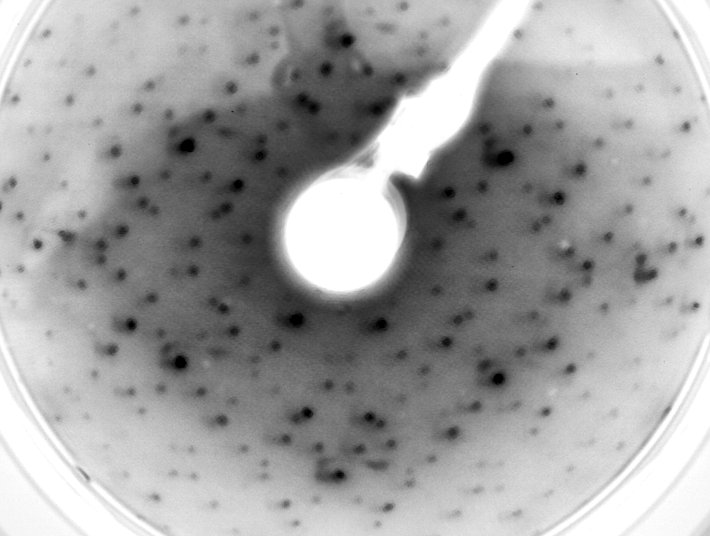
\includegraphics[width=\textwidth]{bilder/unbedampft_E207_MitteKristall.jpg}
	\caption*{Mitte des Kristalls}
	\end{minipage}
\end{figure}
\end{frame}

\begin{frame}
\frametitle{LEED des Re-Kristalls}
\vspace{-0.2cm}
\begin{figure}[H]
\begin{minipage}[b]{0.45\textwidth}
\includesvg[svgpath=bilder/]{unbedampft_E207-winkel}
\end{minipage}
\begin{minipage}[b]{0.45\textwidth}
\includesvg[svgpath=bilder/]{bcc-hcp}
\end{minipage}
\caption*{a) Eingezeichnete größt- und
kleinstmögliche Winkel.\\ b) (0001)-Oberfläche der hcp-Struktur, $\alpha=120^{\circ}$ und
$\beta=60^{\circ}$.\\ c) (110)-Oberfläche der bcc-Struktur, $\alpha\approx109{,}5^{\circ}$ und
$\beta\approx70{,}5^{\circ}$.}
\end{figure}
\vspace{-0.5cm}
\small\begin{table}[H]
\centering
\begin{tabular}{ c  r  r  r}
Winkel &	min	 &	max & Mittel \\
 \hline                       
 $\alpha$&105,8$^{\circ}$&111,4$^{\circ}$&108,6$^{\circ}$\\
 $\beta$&71,5$^{\circ}$&74,4$^{\circ}$&73,0$^{\circ}$\\
 $\gamma$&106,7$^{\circ}$&112,9$^{\circ}$&109,8$^{\circ}$\\
 $\delta$&67,2$^{\circ}$&73,1$^{\circ}$&70,2$^{\circ}$\\
\end{tabular}
\end{table}
\end{frame}

\begin{frame}
\frametitle{LEED des bedampften Re-Kristalls}
\begin{minipage}{\linewidth}
%\vspace{-0.4cm}
\begin{figure}[H]
		\captionsetup{name=Abb.}
	\begin{minipage}[b]{0.3\textwidth} 
		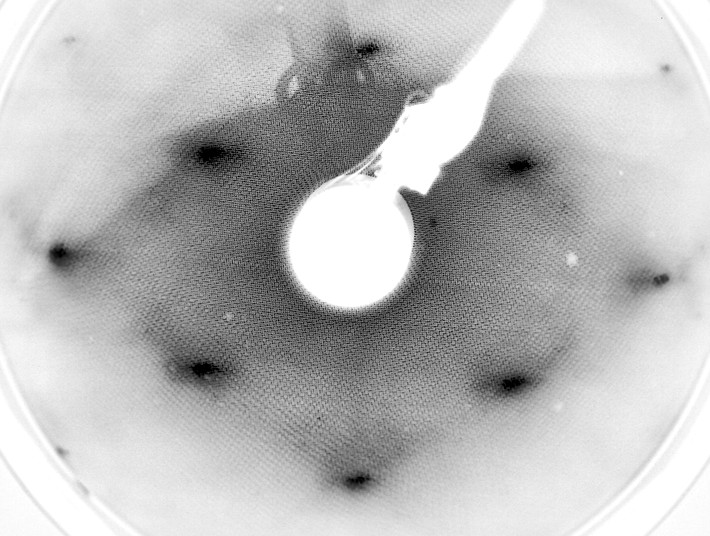
\includegraphics[width=\textwidth]{bilder/unbedampft_E207}
		\caption*{\textit{Re-Oberfläche}}
	\end{minipage}
	\hfill
	\begin{minipage}[b]{0.3\textwidth}
		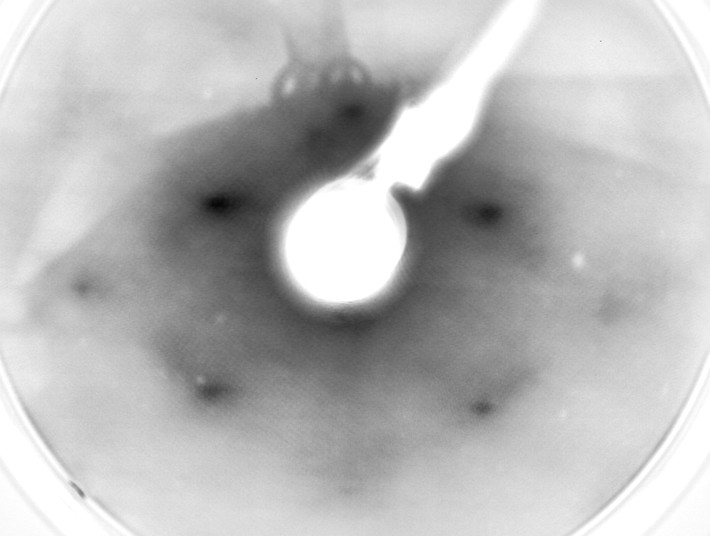
\includegraphics[width=\textwidth]{bilder/0_5ML_E208}
		\caption*{\textit{1/2 Monolage Au}} 
	\end{minipage}
	\hfill
	\begin{minipage}[b]{0.3\textwidth} 
		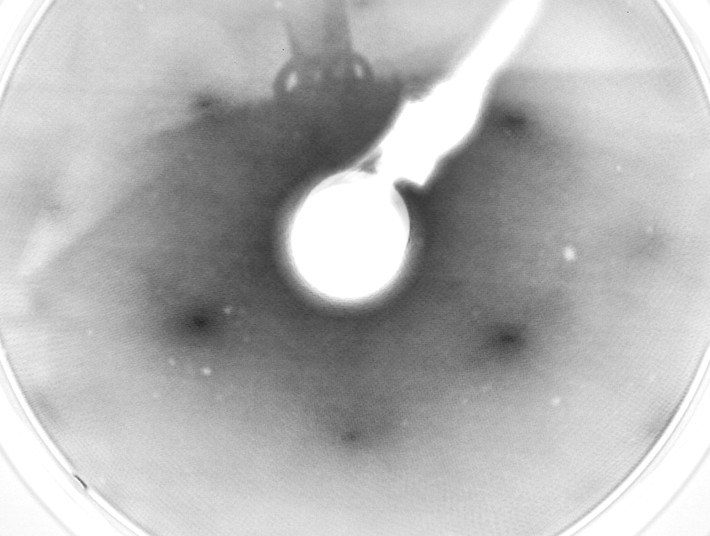
\includegraphics[width=\textwidth]{bilder/1ML_E207}
		\caption*{\textit{1 Monolage Au}} 
	\end{minipage}
	
	\begin{minipage}[b]{0.3\textwidth}
		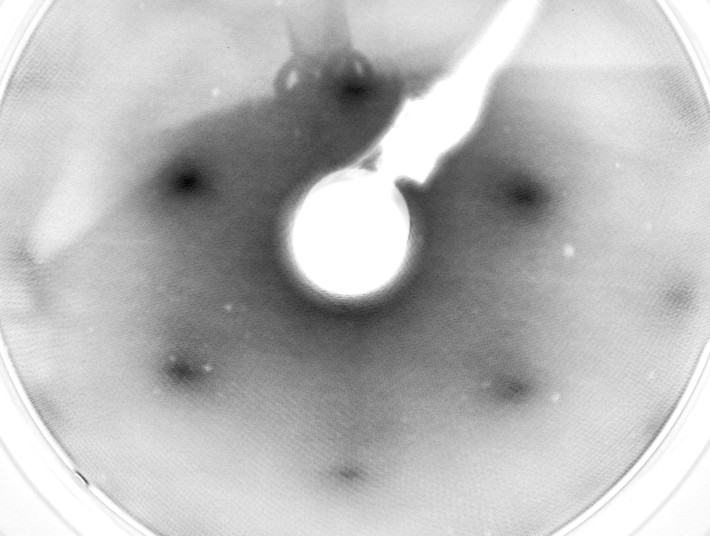
\includegraphics[width=\textwidth]{bilder/6ML_E207}
		\caption*{\textit{6 Monolagen Au}}
	\end{minipage}
	\hfill
	\begin{minipage}[b]{0.3\textwidth} 
		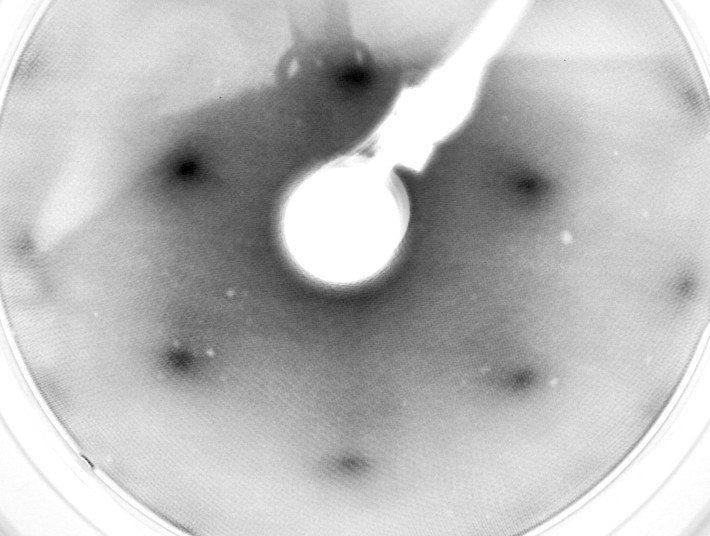
\includegraphics[width=\textwidth]{bilder/10ML_E207}
		\caption*{\textit{10 Monolagen Au}}
	\end{minipage}
	\hfill
	\begin{minipage}[b]{0.3\textwidth}
		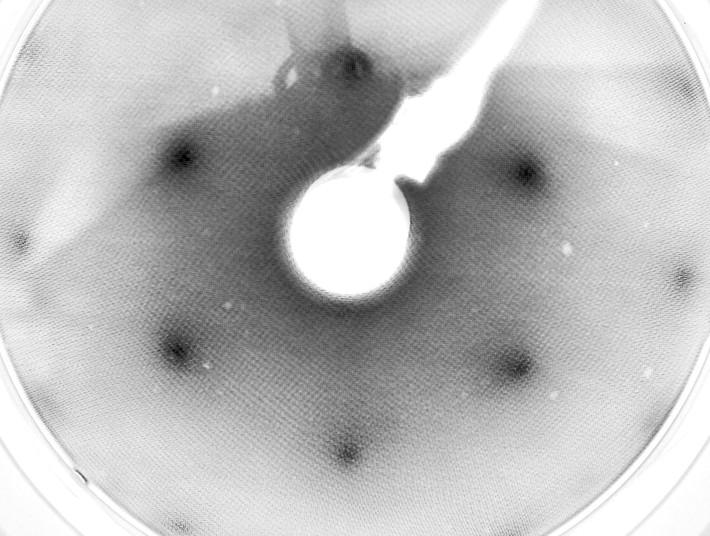
\includegraphics[width=\textwidth]{bilder/30ML_E208}
		\caption*{\textit{30 Monolagen Au}}
	\end{minipage}
% 	\caption*{LEED-Aufnahmen vom Re-Kristall ohne
% 	und mit verschiedenen Bedeckungsgraden von Gold bei einer Elektronenenergie von \SI{208}{eV}.}
\end{figure}
\end{minipage}
\end{frame}

%___________________________________________________________________________________________________________________________________________
%___________________________________________________________________________________________________________________________________________


\subsection[Ergebnisse]{STM}

\begin{frame}
\frametitle{STM des Re-Kristalls}
\begin{figure}[htbp]
	\vspace{-0.5cm}
	\begin{minipage}[b]{0.45\textwidth} 
		\sffamily
		\includesvg[svgpath=bilder/]{rekristall1}
	\end{minipage}
	\hspace{0.5cm}
	\begin{minipage}[b]{0.45\textwidth}
		\sffamily
		\includesvg[svgpath=bilder/]{rekristall2}
	\end{minipage}
	\caption*{Regelmäßig angeordnete Terrassen, Breite etwa \SI{35}{nm}}
	\end{figure}
\end{frame}

\begin{frame}
\frametitle{STM halbe Monolage Au}
\begin{figure}
\begin{minipage}[b]{0.45\textwidth} 
		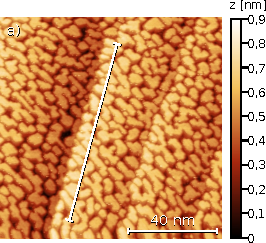
\includegraphics{bilder/profilhalbeMLkleiner}
	\end{minipage}
	\begin{minipage}[b]{0.45\textwidth}
		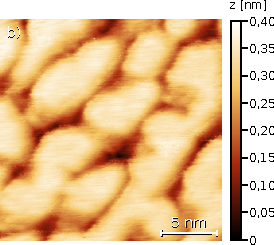
\includegraphics{bilder/halbeMLkleiner}
	\end{minipage}
% 	\caption{\textit{STM-Bilder von 0,5 Monolagen Gold auf Re. Es bilden sich Inseln aus
% 	mehreren Goldatomen von einer Größe von etwa \SI{7}{nm} Länge, die die Re-Oberfläche ungeordnet bedecken.}}
	\vfill
	\centering
	\vspace{0.3cm}\hspace{-1.5cm} 
	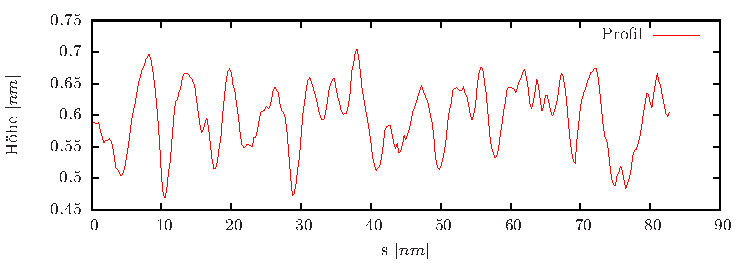
\includegraphics[height=3cm]{bilder/ProfilhalbeML.pdf}
% 	\caption{\textit{Höhenprofil aus Abb. \ref{halbeML2stm}a). Die Höhe der Goldinseln liegt bei etwa
% 	\SI{0,2}{nm}.}}
\end{figure}
\end{frame}

\begin{frame}
\frametitle{STM mehrere Monolagen Au}
\begin{figure}[H]
	\begin{minipage}[b]{0.45\textwidth} 
		\includesvg[svgpath=bilder/]{20ML}
	\end{minipage}
% 	\caption*{20 Monolagen Gold}
	\hspace{0.5cm} 
	\begin{minipage}[b]{0.45\textwidth}
		\includesvg[svgpath=bilder/]{30ML}
	\end{minipage}
% 	\caption*{30 Monolagen Gold}
\caption*{20 Monolagen Gold~~~~~~~~~~~~~~~~~~~~~~~~~~~~~~~~~~~~~~30 Monolagen Gold}
\end{figure}
\end{frame}

\begin{frame}
\frametitle{STM 20 Monolagen}
\vspace{-0.3cm}
\begin{figure}[H]
	\begin{minipage}[b]{0.45\textwidth} 
		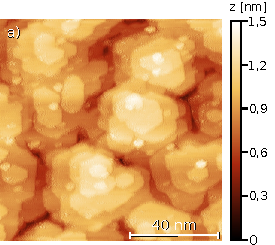
\includegraphics{bilder/20ML_2kleiner}
		\caption*{20 ML ungetempert}
	\end{minipage}
	\hspace{0.5cm} 
	\begin{minipage}[b]{0.45\textwidth}
		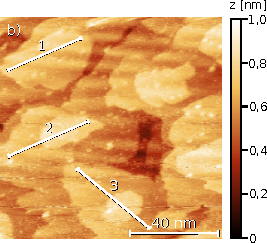
\includegraphics{bilder/20MLget2kleiner}
		\caption*{20 ML \SI{10}{min} getempert bei \SI{2,0}{A}}
	\end{minipage}
% 	\caption{\textit{a) 20 Monolagen ungetempert, b) 20 Monolagen, 10 Minuten mit einem Filamentstrom
% 	von \SI{2,0}{A} getempert.
% 	Beim Tempern glättet sich die Oberfläche, es bilden sich größere, flache Inseln.}}
	\centering
		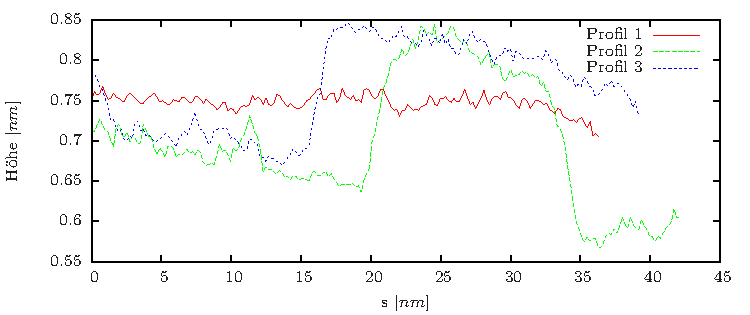
\includegraphics[height=3cm]{bilder/profiles20MLget}
% 	\caption{\textit{Höhenprofil aus Abb. \ref{getVergleich}b). Die Höhen der Oberflächen der Inseln
% 	schwanken im Bereich von etwa \SI{0,05}{nm}, somit sind die Inseln sehr eben.}}
\end{figure}
\end{frame}

\begin{frame}
\frametitle{Zusammenfassung}
%\framesubtitle{Subtitles are optional}
\begin{itemize}\setlength{\itemsep}{+15pt}
  \item Art des Wachstums nicht eindeutig, aber:
  \item 30 Monolagen als Molekülsubstrat geeignet
  \item gleiches Ergebnis für 20 Monolagen getempert: ca. \SI{30}{nm} bis \SI{35}{nm} im Durchmesser
  große, glatte Inseln
  \item periodische angeordnete Oberfläche (LEED)
  \item genügend große Flächen, um Anordnung von aufgebrachten organischen Molekülen zu untersuchen
\end{itemize}
\end{frame}


%___________________________________________________________________________________________________________________________________________
%___________________________________________________________________________________________________________________________________________
%___________________________________________________________________________________________________________________________________________


\section{Aufbau und Test einer Spraydepositionsapparatur}

%___________________________________________________________________________________________________________________________________________
%___________________________________________________________________________________________________________________________________________


\begin{frame}
\frametitle{}
%\framesubtitle{Subtitles are optional}
\begin{center}
\textcolor{darkred}{\huge{2. Teil:\\ \vspace{0.65cm}
 Aufbau und Test einer\\ \vspace{0.5cm}Spraydepositionsapparatur}}
\end{center}


\end{frame}

%___________________________________________________________________________________________________________________________________________
%___________________________________________________________________________________________________________________________________________


\subsection[Motivation]{Einleitung}

\begin{frame}
\frametitle{Wozu das Ganze?}
%\framesubtitle{Subtitles are optional}
\begin{itemize}\setlength{\itemsep}{+15pt}
  \item Funktioniert über ein Druckgefälle innerhalb der Apparatur
  \item Moleküle in Lösung werden auf Substrat "`gesprüht"'
  \item Vorteil: kein thermisches Verdampfen $\Rightarrow$ keine Verformung der Moleküle
\end{itemize}
\end{frame}

%___________________________________________________________________________________________________________________________________________
%___________________________________________________________________________________________________________________________________________


\subsection[Versuchsaufbau]{Versuchsaufbau}

\begin{frame}
\frametitle{Schema der Spraydepositionsapparatur}
\begin{figure}[H]
\centering
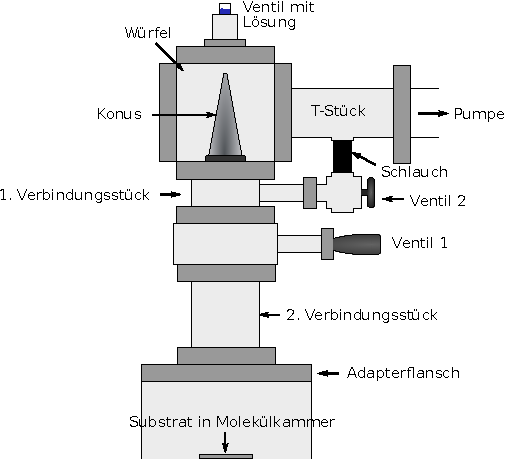
\includegraphics{bilder/wuerfelklein.pdf}
\end{figure}
\end{frame}

\begin{frame}
\frametitle{Aufbau der Apparatur (1)}
%\framesubtitle{Subtitles are optional}
\begin{itemize}\setlength{\itemsep}{+15pt}
  \item Test an HV-Apparatur inkl. Vorpumpe $\&$ Hauptpumpe, Druckmessgerät (Vorteil kleineres
  Volumen)
  \item Substrat: Glasträger
  \item gelöste Moleküle: \\
  Kupfer-2-Phthalocyanin (CuPc) in Dimethylsulfoxid bzw. Dimethylformamid\\
  Tetracyanoquinodimethan (TCNQ) in Tetrahydrofuran
\end{itemize}
\end{frame}


\begin{frame}
\frametitle{Aufbau der Apparatur (2)}
\begin{figure}[H]
\centering
%\sffamily
\includesvg[svgpath=bilder/]{sb}
\end{figure}
\end{frame}

%___________________________________________________________________________________________________________________________________________
%___________________________________________________________________________________________________________________________________________


\subsection[Ergebnisse]{Test der Apparatur}

\begin{frame}
\frametitle{Erste Tests}
%\framesubtitle{Subtitles are optional}
\begin{itemize}\setlength{\itemsep}{+15pt}
  \item Getestete Zeiten: \\
  \SI{1}{ms} bis \SI{50}{ms} offenes Ventil ("`On-Time"'), dazwischen \SI{7}{ms} bis \SI{4}{s} geschlossenes
  Ventil ("`Off-Time"')\\ 
  gesamte Zyklusdauer bis 15 Minuten
  \item Druckanstieg in der Hauptkammer, aber nichts zu sehen auf Glasträger!
  \item Nach einigen Umbauten: Sichtbare farbige Spritzer auf Glasträger erst ohne Pumpe am Würfel
\end{itemize}
\end{frame}


\begin{frame}
\frametitle{Beobachtungen zwischendrin}
%\framesubtitle{Subtitles are optional}
\begin{itemize}\setlength{\itemsep}{+15pt}
  \item Ausgangsdruck in Hauptkammer \SI{e-5}{mbar} $\Rightarrow$ Druckanstieg bei Öffnen des
  Ventils auf \SI{e-3}{mbar}\\
  Druck in Würfel nur \SI{e-2}{mbar}
 % einigermaßen regulierbar über kurze On-, lange Off-Zeiten
  \item Öffnungen von Ventil $\&$ Konus anfällig für Verstopfungen $\Rightarrow$ kein Druckanstieg
  mehr in Hauptkammer
  \item Turbopumpe stark am Limit:\\
  Austausch der internen Vorpumpe durch externe Membranpumpe
\end{itemize}
\end{frame}

\begin{frame}
\frametitle{Test mit Quarzwaage}
%\framesubtitle{Subtitles are optional}
\begin{itemize}\setlength{\itemsep}{+15pt}
  \item Einbau von Quarzwaage statt Glasträger
  \item Beobachtung der relativen Frequenzänderung mit digitaler Anzeige
  \item On-Time von \SI{3}{ms}, Off-Time von \SI{500}{ms} (fast kein Anstieg des Drucks in der
  Hauptkammer)
  \item Anstieg von $30\pm1$ SKT in \SI{30}{min}
  \item bei nachfolgender Reinigung: Abfall um $15\pm1$ SKT \\
  $\Rightarrow$ Nettozunahme um $15\pm1$ SKT \\
  $\Rightarrow$ Deposition der Moleküle auf Quarz
\end{itemize}
\end{frame}

%___________________________________________________________________________________________________________________________________________
%___________________________________________________________________________________________________________________________________________
%___________________________________________________________________________________________________________________________________________



\section{Zusammenfassung}

\begin{frame}
\frametitle<presentation>{Alles in allem\ldots}

\begin{itemize}\setlength{\itemsep}{+15pt}
  \item Gold auf Rhenium:\vspace{0.5cm}
  		\begin{itemize}\setlength{\itemsep}{+7pt}
  		  \item  Inselwachstum 
  		  \item  20-30 Monolagen ausreichend
  		  \item  durch Tempern Glättung der Oberfläche
  		\end{itemize}
  \item Spraydepositionsapparatur:\vspace{0.5cm}
    	\begin{itemize}
  		  \item  Scheint zu funktionieren!	  
  		\end{itemize}
\end{itemize}
\end{frame}

\section*{Ausblick}

\begin{frame}
\frametitle<presentation>{Was bleibt zu tun?}
% The following outlook is optional.
Weitere Tests!
\vspace{0.5cm}
\begin{itemize}\setlength{\itemsep}{+15pt}
  \item Wieviele SKT sind wieviele Moleküle?
  \item Verdampft das Lösungsmittel?
  \item Wie stark muss man die Lösung verdünnen?
  \item Was kann man am Druck verbessern?
  \item Behalten die Moküle bei dieser Methode ihre Form?
  \item \ldots
  
\end{itemize}
\end{frame}

\end{document}
